\section{MATERIALS AND METHODS}

\subsection{Data, preprocessing, and split}
Data were collected from point measurements in Lago do Serpa (Itacoatiara, AM) and organized in CSV with
coordinates ($x, y$) and physicochemical variables (\textit{pH}, dissolved oxygen, temperature, apparent color,
turbidity, and true color). Cleaning included decimal separator conversion, numerical consistency checks,
and removal of incomplete rows. Inputs were defined as $x, y, TEMP, COR\_A,$ and COR\_V; in the univariate
model the output was pH, while in the multimodal model the outputs were pH, dissolved oxygen, and turbidity,
without including target variables as inputs to avoid leakage. The dataset was georeferenced in Lago do Serpa
(Figure~\ref{fig:mapa_pontos}), and to mitigate overfitting in a small dataset we applied \textbf{synthetic data
augmentation} (factor 10) with light Gaussian noise to stabilize training.


\begin{figure}[!t]
	\centering
	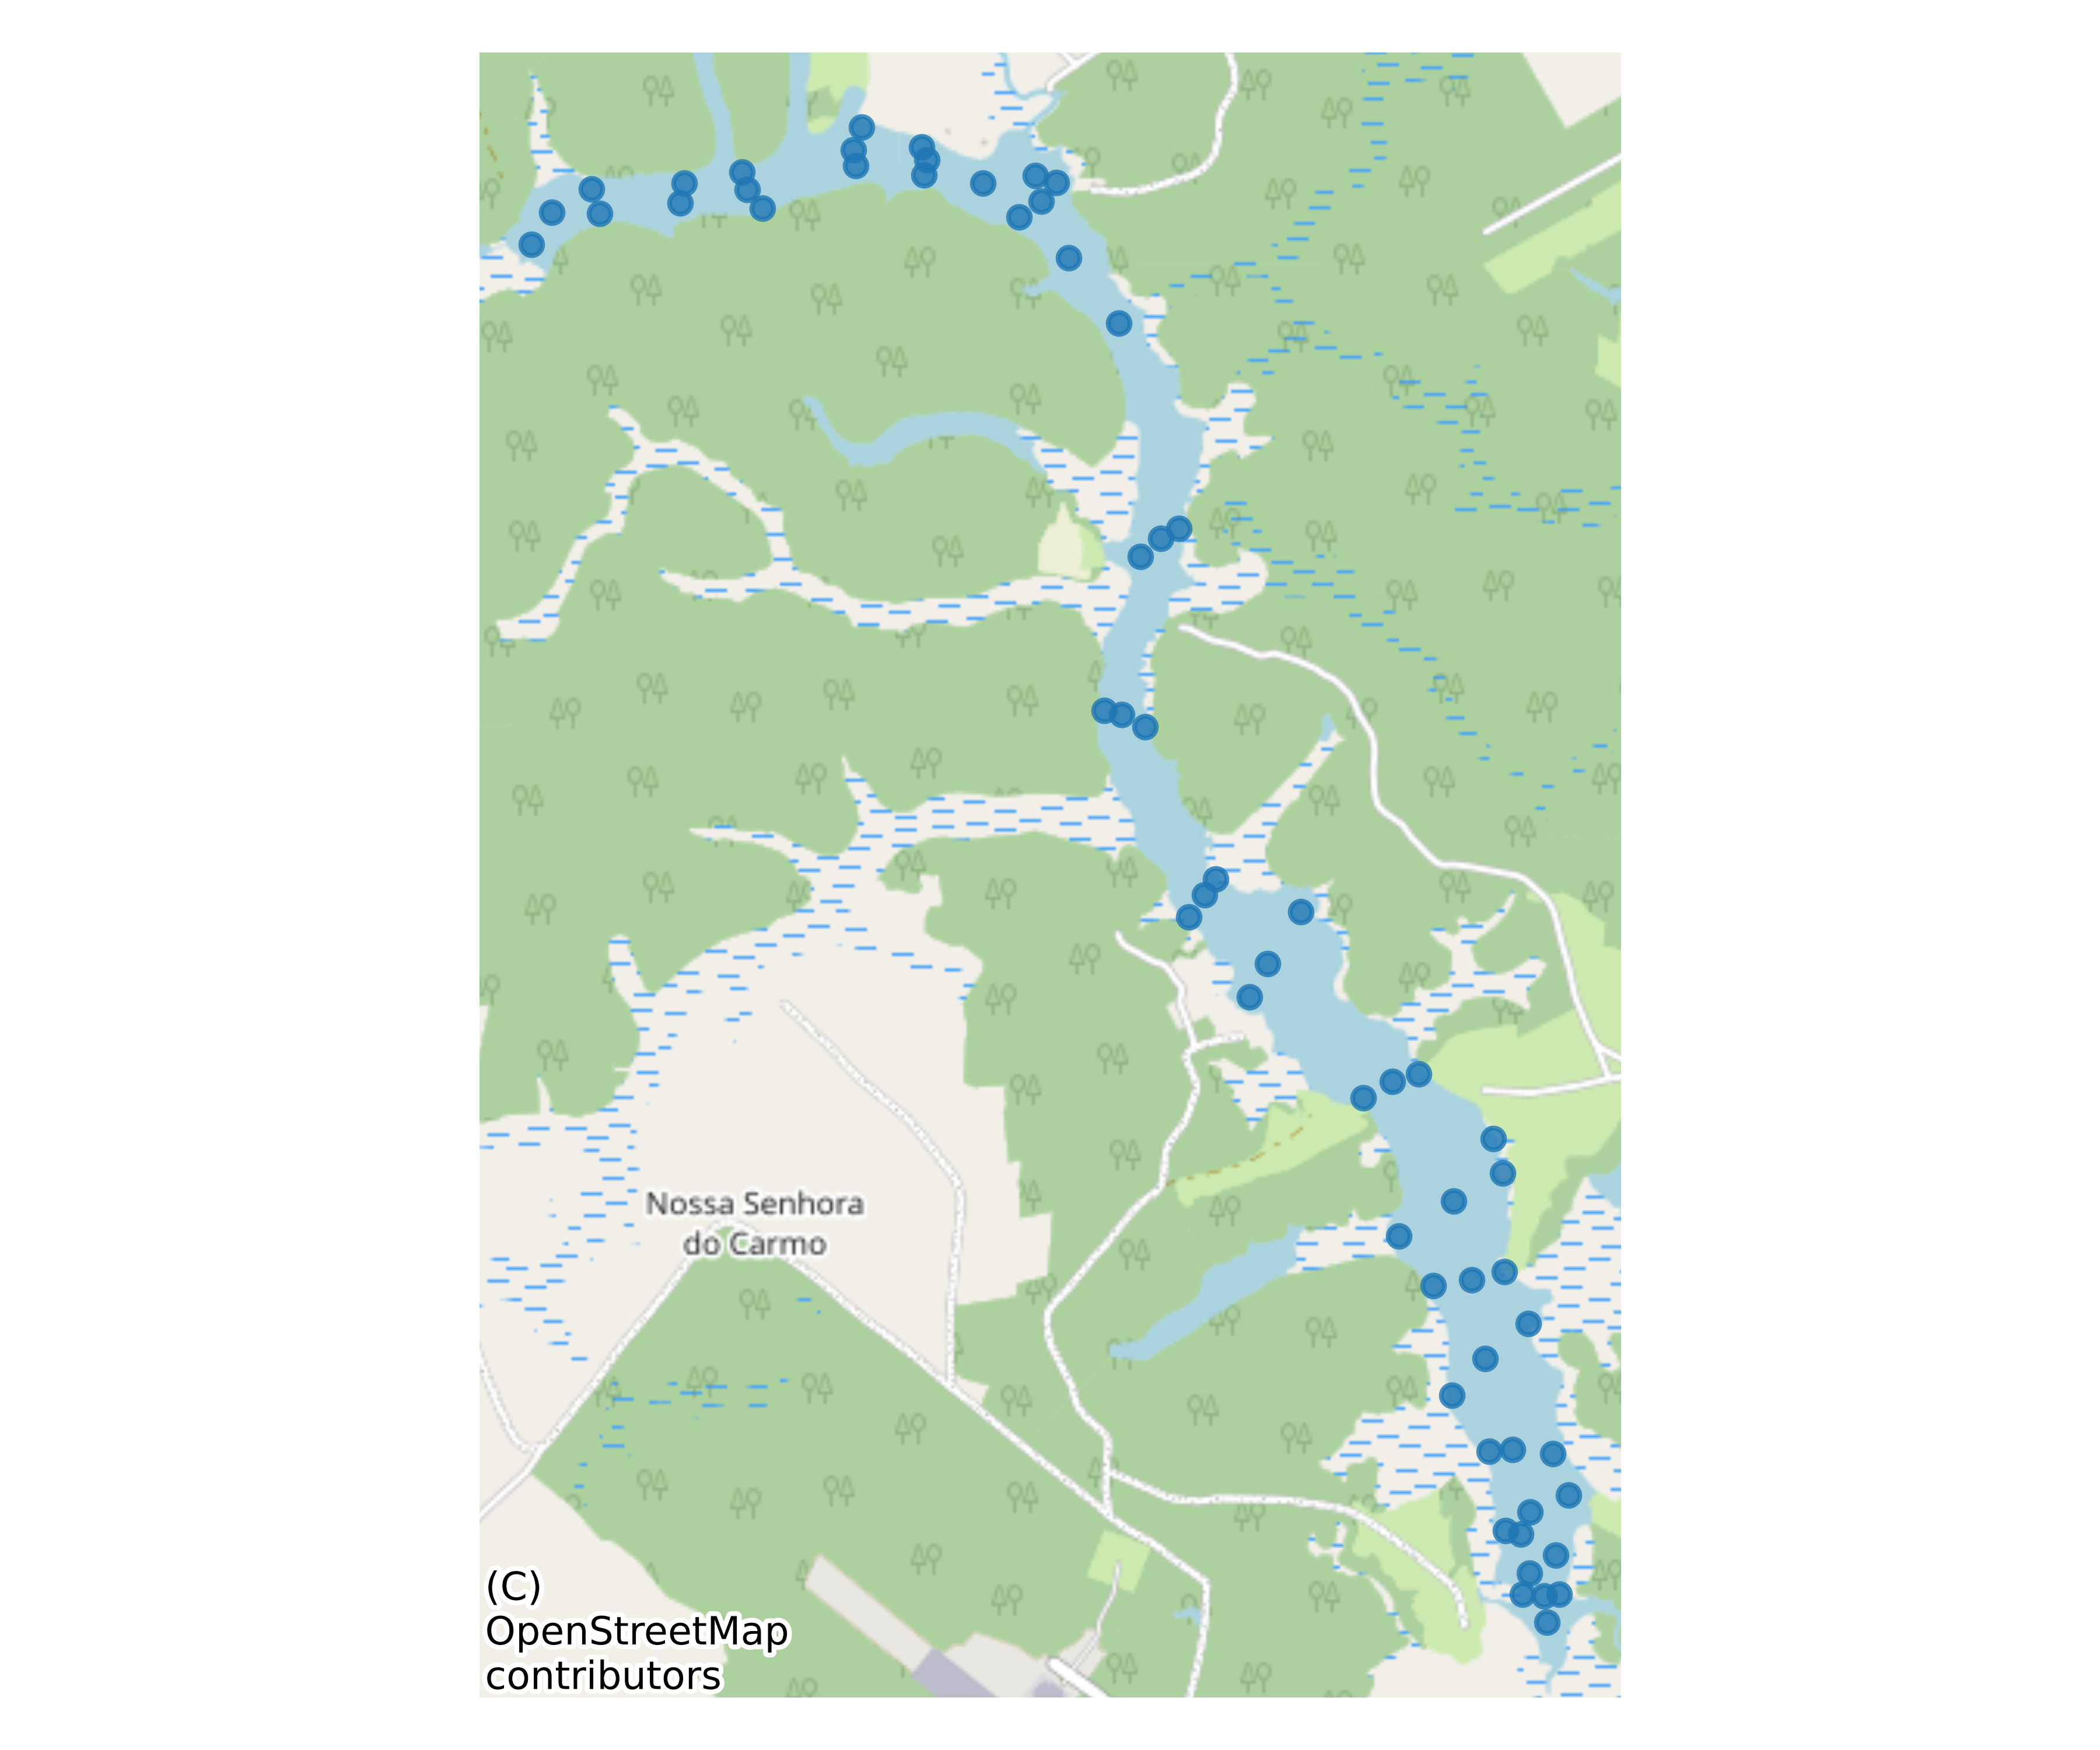
\includegraphics[width=0.75\textwidth]{./figuras/map_points_osm_21S.png}
\caption{Sampling locations in Lago do Serpa (Itacoatiara, AM) on an OpenStreetMap basemap.
Coordinates were converted to latitude/longitude (WGS84, UTM 21S).}
	\label{fig:mapa_pontos}
\end{figure}
\FloatBarrier

Inputs were normalized via z-score using training statistics; multimodal outputs were optionally normalized. The
train/validation/test split used fixed proportions with seed-controlled shuffling. This split (Table~\ref{tab:data_split})
is used in all experiments.

\begin{table}[H]
\centering
\caption{Dataset split.}
\begin{tabular}{lcc}
\toprule
Split & Proportion & Number of samples \\
\midrule
Train & 70\% & 42 \\
Validation & 10\% & 6 \\
Test & 20\% & 12 \\
\bottomrule
\end{tabular}
\label{tab:data_split}
\end{table}




\subsection{Modeling, training, and evaluation}
Normalized inputs were encoded into spike trains using \textit{rate coding}, where firing probability is a
sigmoidal function of the input. The SNN used a dense input layer, a hidden layer with Leaky Integrate-and-Fire
(LIF) neurons, and a linear output layer. Inference runs over $T$ time steps, accumulating hidden activity,
which enables sparse processing; larger $T$ increases temporal resolution but also latency and power consumption.
Training used Adam and MSE with \textit{early stopping} and grid search over $T$, learning rate, threshold,
decay, and hidden size, as well as augmentation noise intensity; the best configuration was selected by the
lowest validation error. For the multimodal model, we used weighted loss and optional target normalization to
predict pH, dissolved oxygen, and turbidity in a single network. From predictions, we defined a composite
pollution index using (i) deviation from neutral pH, (ii) inverse dissolved oxygen, and (iii) normalized
turbidity; CONAMA Resolution 357/2005 is used as a \textbf{normative reference} to interpret estimated levels,
without replacing official indices \cite{conama3572005}. The index was categorized into three relative levels:
low ($[0,0{,}33)$), medium ($[0{,}33,0{,}66)$), and high ($[0{,}66,1]$). Exploratory analyses included boxplots
and correlations, while spatial interpretation used point maps and inverse-distance weighting (IDW) surfaces
for pH, dissolved oxygen, turbidity, and the pollution index. Model comparison used a multiseed benchmark and
a paired sign test on macro metrics, suitable for small samples without normality assumptions.

\subsection{Export and mobile deployment}
After final training, the multimodal model was exported for mobile inference by serializing PyTorch
weights, converting to ONNX while preserving the input/output signature, and transforming to TensorFlow
Lite (TFLite) for a lightweight Android runtime. In the Flutter app, the \textit{.tflite} model and
normalization parameters (mean and standard deviation) are loaded at startup so each sample is normalized
locally before being passed to the TFLite interpreter. Model outputs (pH, dissolved oxygen, turbidity)
are de-normalized and used to compute the composite pollution index in real time. For field operations
without connectivity, the map is shown offline using MBTiles (Mapbox Tiles), preserving spatial context
without internet access.

\subsection{Architecture and integration}
To assess neuromorphic feasibility on constrained hardware, this study focused on implementing and
analyzing SNNs on edge devices. The goal was to evaluate efficiency and accuracy under memory,
processing, and energy constraints typical of edge deployment. The proposed SNN uses Leaky Integrate-and-Fire
(LIF) neurons to optimize sparse event processing. The architecture (Figure~\ref{fig:minhafigura}) organizes
the flow into Input, Processing, and Output stages, exploiting temporal sparsity and activating computation
mainly when relevant changes occur, which favors energy efficiency in autonomous systems.

At the Input stage, Lago do Serpa data are normalized (z-score) and augmented to stabilize training.
The neuromorphic stage performs temporal encoding (\textit{rate coding}) to convert scalar values into
spike trains and runs LIF-based inference. Optimization includes weight and hyperparameter tuning (grid
search and \textit{early stopping}), guided by the loss function. After training, the model is exported
via PyTorch $\rightarrow$ ONNX $\rightarrow$ TFLite for edge deployment. In operation, the same model
runs offline on smartphones, Raspberry Pi, and ESP32, producing multimodal predictions (pH, dissolved
oxygen, turbidity), a pollution index, and spatial maps to support field decision-making.

\begin{figure}[ht!] 
	\centering
	\caption{ 
		Proposed neuromorphic architecture for water-quality prediction, highlighting input
		and preprocessing, neuromorphic training with SNN (LIF) and \textit{rate coding}, the
		PyTorch $\rightarrow$ ONNX $\rightarrow$ TFLite export pipeline, and offline deployment
		on edge devices.
	}
	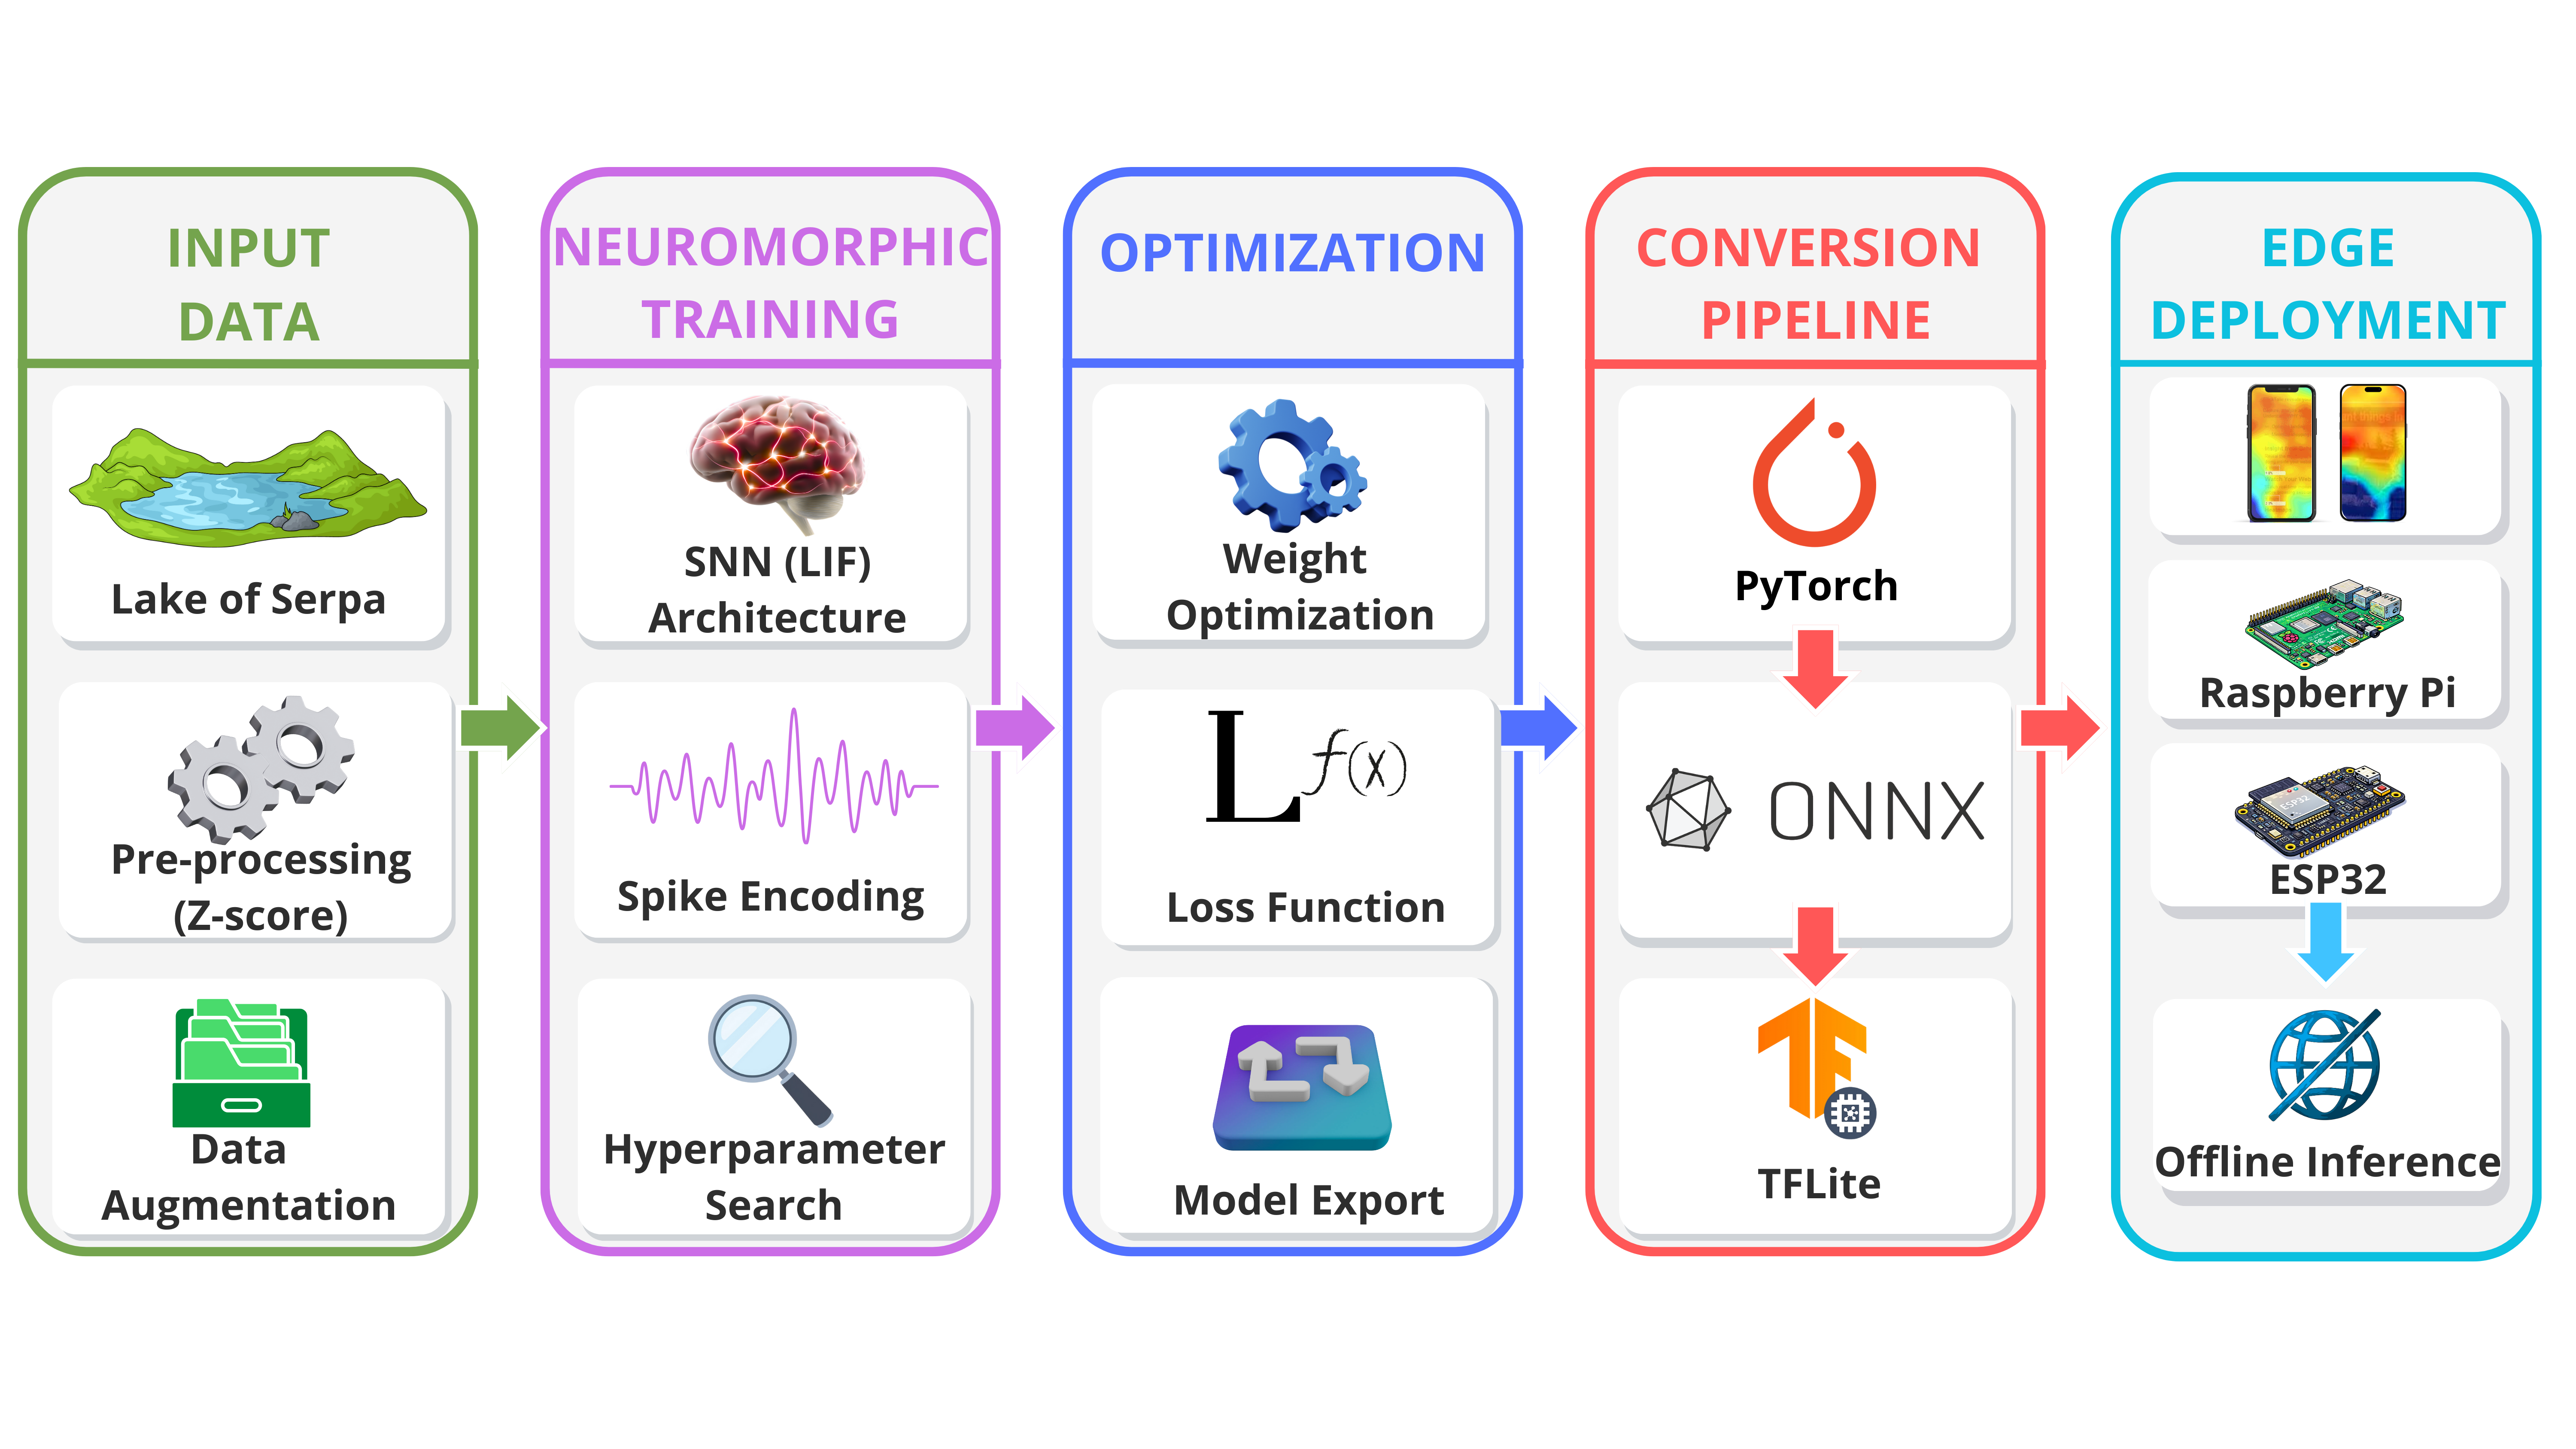
\includegraphics[width=0.8\textwidth]{./figuras/Arquitetura.png}
	\centering
	
	\label{fig:minhafigura}
\end{figure}

\FloatBarrier
\subsection{Hardware specifications for training and inference}

To ensure experimental reproducibility and effective validation, a dedicated workstation was used for
development, offline training, and preliminary inference simulations. Hardware and software specifications
are listed in Table~\ref{tab:hardware}.

\begin{table}[H]
\centering
\caption{Workstation specifications used in the experiments.}
\begin{tabular}{ll}
\toprule
Component & Specification \\
\midrule
CPU & Intel(R) Core(TM) i7-14650HX (24 threads) \\
Memory & 15 GiB \\
GPU & NVIDIA GeForce RTX 4060 (8 GB VRAM), Driver 550.163.01, CUDA 12.4 \\
Operating System & Ubuntu 22.04.5 LTS (64-bit) \\
\bottomrule
\end{tabular}
\label{tab:hardware}
\end{table}

This environment enabled efficient training with surrogate gradients, which are essential to handle
spike non-differentiability prior to portability and optimized deployment on edge devices.

To characterize low-power inference feasibility, the TFLite model was executed on a Raspberry Pi 4B
(ARM64) with the XNNPACK delegate (TFLite kernel optimizer), following the export pipeline described
in Section 3.7. Device specifications are listed in Table~\ref{tab:hardware_rpi}.

\begin{table}[H]
\centering
\caption{Inference device specifications (Raspberry Pi 4B).}
\begin{tabular}{ll}
\toprule
Component & Specification \\
\midrule
Board & Raspberry Pi 4B \\
Architecture & ARM64 \\
Operating System & Linux 6.12.34+rpt-rpi-v8-aarch64 \\
Runtime & TFLite (delegate XNNPACK) \\
\bottomrule
\end{tabular}
\label{tab:hardware_rpi}
\end{table}

Additionally, to evaluate execution on mobile edge devices, the Android app was tested on three phones:
\textit{23021RAAEG} (Qualcomm SoC, Android 15, MemTotal: 5.77 GB), \textit{SM-A566E} (s5e8855 SoC,
Android 16, MemTotal: 7.60 GB), and \textit{2201117SG} (mt6781 SoC, Android 13, MemTotal: 5.86 GB).
These configurations were used for latency benchmarks in the app.

\subsection{Energy measurement}
To quantify incremental energy during inference, an INA219 current sensor was placed in series with
the device power supply and sampled over I\textsuperscript{2}C. Telemetry was recorded periodically
and smoothed with an exponential moving average (EMA), while energy was accumulated over time from the
EMA power estimate. Two windows were considered: \textit{idle} (device idle) and \textit{load}
(inference benchmark). Average power was computed as $P = V \cdot I$, incremental power as
$\Delta P = P_{load} - P_{idle}$, and energy per inference as $\Delta P / \mathrm{throughput}$,
yielding mJ/inf for cross-platform comparison.

\begin{algorithm}[H]
\caption{Energy measurement procedure using the INA219 sensor.}
\begin{algorithmic}[1]
\STATE \textbf{Initialization:}
\STATE Configure INA219 and I\textsuperscript{2}C (calibration 32V/2A).
\STATE Initialize serial communication at 9600 baud.
\STATE Set telemetry period $\Delta t = 500$ ms and EMA coefficient $\alpha = 0.2$.
\STATE \textbf{Real-time sampling:}
\WHILE{running}
\STATE Read bus voltage $V(t)$ and current $I(t)$ from INA219.
\STATE Compute instantaneous power $P(t) = V(t)\cdot I(t)$.
\STATE Update EMA power: $P_{EMA}(t) = \alpha P(t) + (1-\alpha)P_{EMA}(t-1)$.
\STATE Accumulate energy: $E = E + P_{EMA}(t)\cdot \Delta t$.
\STATE Send $(V(t), I(t), P_{EMA}(t), E)$ over serial.
\ENDWHILE
\STATE \textbf{Energy computation (host):}
\STATE Compute mean idle power $\overline{P}_{idle}$ and mean load power $\overline{P}_{load}$.
\STATE Compute $\Delta P = \overline{P}_{load} - \overline{P}_{idle}$ and $E_{inf} = \Delta P / \text{throughput}$.
\end{algorithmic}
\end{algorithm}

For mobile devices, energy was estimated directly in the Android app. Current was obtained via
\textit{BatteryManager} (\texttt{BATTERY\_PROPERTY\_CURRENT\_NOW}) and voltage via
\textit{ACTION\_BATTERY\_CHANGED} (\texttt{EXTRA\_VOLTAGE}), sampled periodically during \textit{idle}
and \textit{load} (benchmark) windows. Power was computed as $P = V \cdot I$ and incremental power as
$\Delta P = P_{load} - P_{idle}$, enabling energy per inference as $\Delta P / \mathrm{throughput}$
from 200 power samples per device.

For the ESP32 (Espressif microcontroller), inference ran in C/C++ (ESP-IDF) with a dedicated benchmark
routine. We performed 10 \textit{warmup runs}, 1000 executions to estimate mean latency and throughput,
and 200 individual samples for standard deviation, as reported in the firmware serial log.

%----------------------------------------------------------------------------------------
%   RESULTADOS
%----------------------------------------------------------------------------------------
